\documentclass[a4paper, 11pt]{book}
%!TeX TS-program = Lualatex 
%!TeX encoding = UTF-8 Unicode 
%!TeX spellcheck = en-US
% !BIB TS-program = bibtex
%\documentclass[draft,english]{book}
%%%%%%%%%%%%%%%%%%%%%%%%%%%%%%%%%%%%%%%%%%%%%%%%%%%%%%%%%%%%%%%%%%%%%
%%%%%%%%%%%%%%%%%%%%%%%%%%%%%%%%%%%%%%%%%%

%\usepackage[utf8]{inputenc}
\usepackage{graphicx}
\graphicspath{{./figures/}}%
\DeclareGraphicsExtensions{.pdf}
\usepackage{geometry}
\geometry{hscale=0.8,vscale=0.8,centering}

\usepackage{pdfpages}
\usepackage[round]{natbib}
%\usepackage{chapterbib}
\bibliographystyle%
  {unsrtnat}%
%\usepackage{wileyvch}
\usepackage[breaklinks]{hyperref}
\author{Perrinet}\title{\Title}
\usepackage{fancyhdr}
\pagestyle{fancy}
\rhead{\href{http://dx.doi.org/10.1002/9783527680863.ch4}{doi:10.1002/9783527680863.ch4}}
\lhead{Parraga (2015) \emph{Perceptual Psychophysics}}

%\includeonly{}
%%%%%%%%%%%%%%%%%%%%%%%%%%%%%%

\begin{document}
%\include{foreword}
%\tableofcontents
%\include{preface}
\frontmatter
\mainmatter
\addtocounter{chapter}{3} % set them to some other numbers than 0
%\part{}
%\chapterauthor{\AuthorA}
\chapter{Perceptual Psychophysics}
%=========================================%
%______________%
%\section*{Abstract}
%\Abstract
%__

\paragraph{BibTex entry}~~\\

This chapter appeared as: %~\citep{Perrinet15sparse}:
\begin{verbatim}

@inbook{Parraga15sparse,
	Author = {Parraga, C. Alejandro},
	Title = {Perceptual Psychophysics},
	Chapter = {4},
	booktitle = {Biologically inspired computer vision},
	Year = {2015}
	Editor = {Crist{\'{o}}bal, Gabriel and Keil, Matthias S. and Perrinet, Laurent U.},
	month = nov,
	isbn = {9783527680863},
	DOI = {10.1002/9783527680863.ch4},
	url={http://onlinelibrary.wiley.com/doi/10.1002/9783527680863.ch4/summary},
	publisher = {Wiley-VCH Verlag GmbH {\&} Co. KGaA},
	}
	
\end{verbatim}

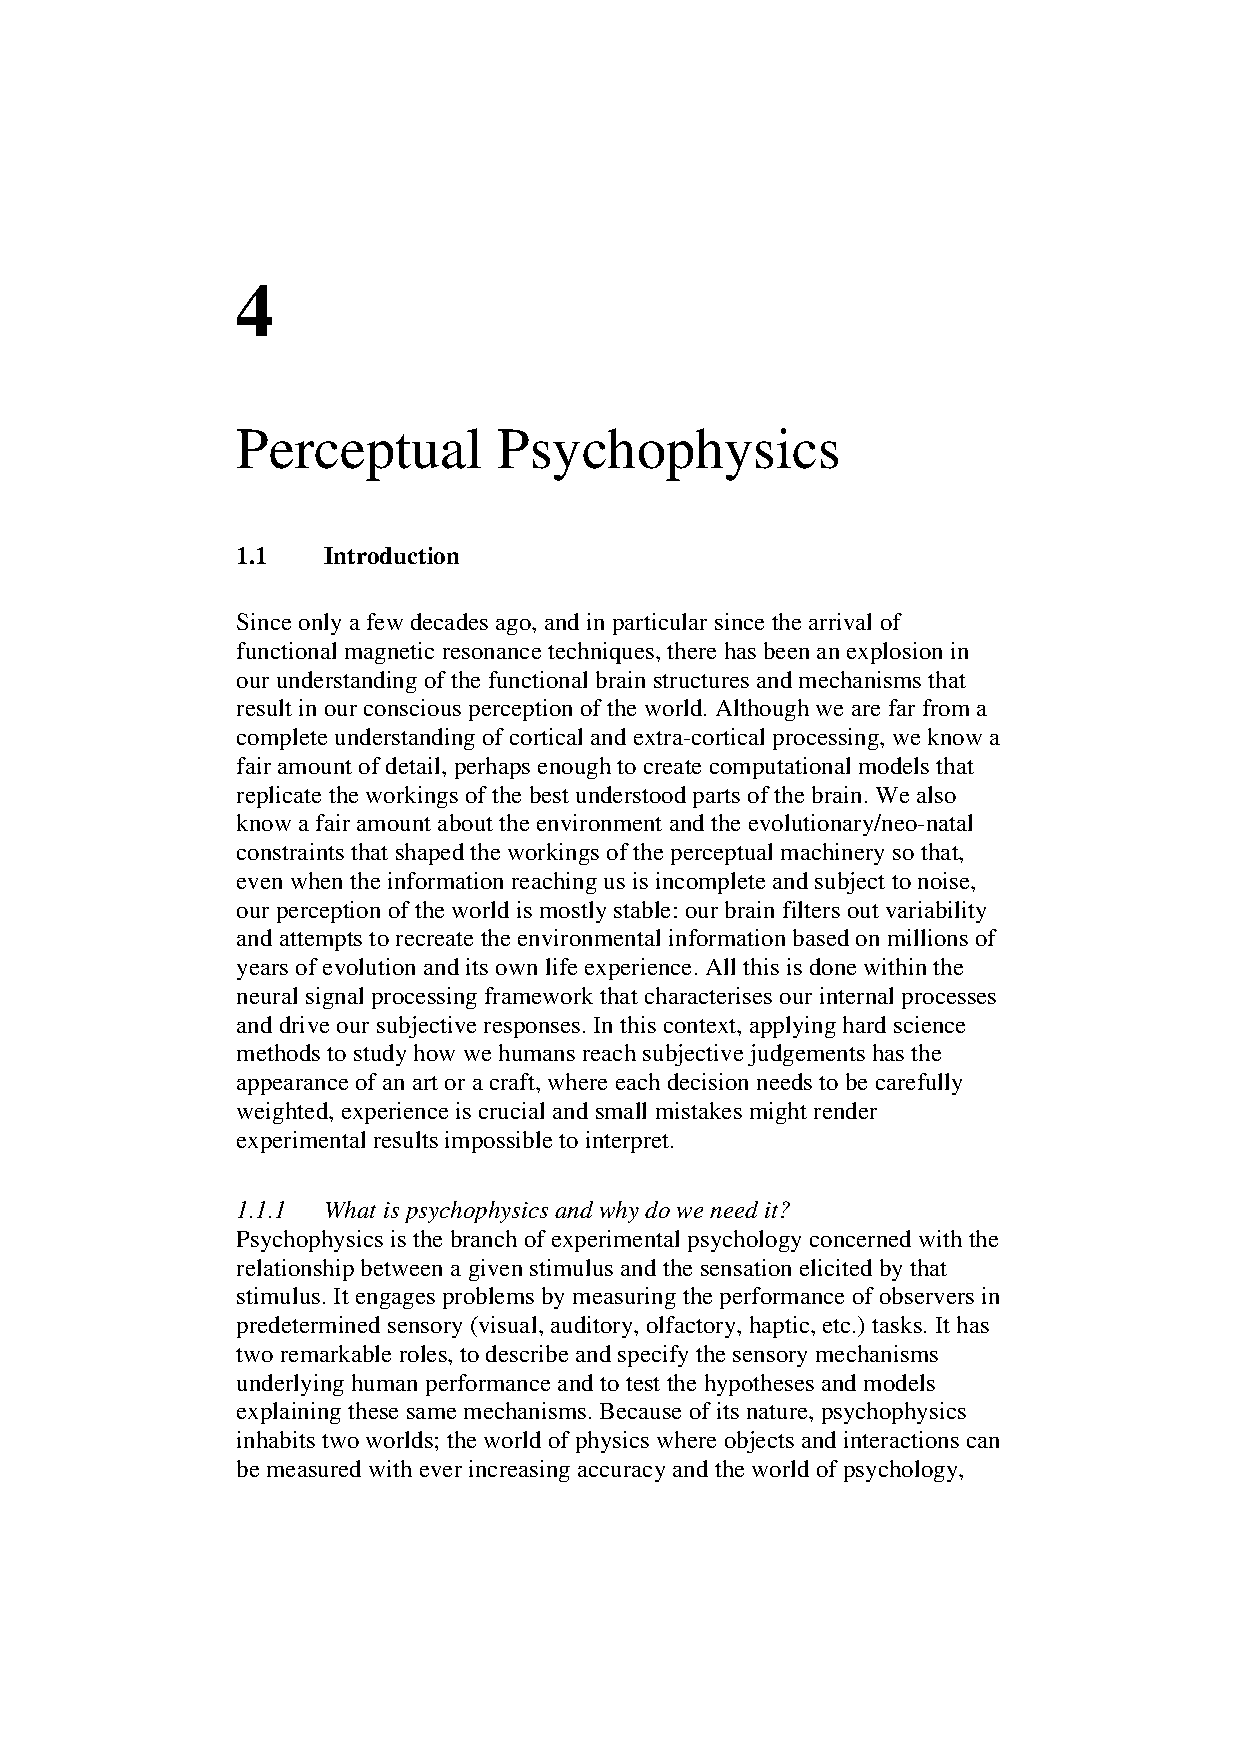
\includepdf[pages=-]{Parraga_Chap4_raw.pdf}

\backmatter

\end{document}
